%%%%%%%%%%%%%%%%%%%%%%%%%%%%%%%%%%%%%%%%
%% MCM/ICM LaTeX Template %%
%% 2022 MCM/ICM           %%
%%%%%%%%%%%%%%%%%%%%%%%%%%%%%%%%%%%%%%%%
\documentclass[12pt]{article}
\usepackage{geometry}
\geometry{left=1in,right=0.75in,top=1in,bottom=1in}

%段落的首行缩进
\usepackage{indentfirst}
\setlength{\parindent}{2em}

%用于表格
\usepackage{makecell}
\usepackage{multirow}

\usepackage{listings}
%%%%%%%%%%%%%%%%%%%%%%%%%%%%%%%%%%%%%%%%
% Replace ABCDEF in the next line with your chosen problem
% and replace 1111111 with your Team Control Number
\newcommand{\Problem}{E}
\newcommand{\Team}{2208269}
%%%%%%%%%%%%%%%%%%%%%%%%%%%%%%%%%%%%%%%%

\usepackage{newtxtext}
\usepackage{amsmath,amssymb,amsthm}
\usepackage{newtxmath} % must come after amsXXX

\usepackage[hidelinks]{hyperref} % 目录添加链接
\usepackage{biblatex} % biblatex
\addbibresource{References.bib}

\usepackage[pdftex]{graphicx}
\usepackage{xcolor}
\usepackage{fancyhdr}
\lhead{Team \Team}
\rhead{}
\cfoot{}

\newtheorem{theorem}{Theorem}
\newtheorem{corollary}[theorem]{Corollary}
\newtheorem{lemma}[theorem]{Lemma}
\newtheorem{definition}{Definition}

%%%%%%%%%%%%%%%%%%%%%%%%%%%%%%%%
\begin{document}
\graphicspath{{.}}  % Place your graphic files in the same directory as your main document
\DeclareGraphicsExtensions{.pdf, .jpg, .tif, .png}
\thispagestyle{empty}
\vspace*{-16ex}
\centerline{\begin{tabular}{*3{c}}
	\parbox[t]{0.3\linewidth}{\begin{center}\textbf{Problem Chosen}\\ \Large \textcolor{red}{\Problem}\end{center}}
	& \parbox[t]{0.3\linewidth}{\begin{center}\textbf{2022\\ MCM/ICM\\ Summary Sheet}\end{center}}
	& \parbox[t]{0.3\linewidth}{\begin{center}\textbf{Team Control Number}\\ \Large \textcolor{red}{\Team}\end{center}}	\\
	\hline
\end{tabular}}
%%%%%%%%%%% Begin Summary %%%%%%%%%%%
% Enter your summary here replacing the (red) text
% Replace the text from here ...
  \bigskip
%改
\centerline{\Large\bfseries More Logging, More Fixed Carbon? Reasonable!}
  \bigskip
  
First, we developed a \textbf{carbon sequestration model} using \textbf{the biomass method}. We decomposed the total carbon sequestration into two parts: forest product sequestration and forest carbon sequestration, and the management strategy into logging strategy and production strategy. We derived the best calculation function for forest biomass by \textbf{curve fitting} and converted it into carbon sequestration. \textbf{Cluster analysis method} is applied to classify forest products for carbon sequestration calculation.

We also innovatively considered the effect of the final destination of trees and forest products (landfill and incineration) on the amount of carbon sequestered. By analyzing the changes of carbon sequestration under different management strategy, we finally derived a model of \textbf{forest carbon sequestration} under specified strategy for forest management measures.(Task1)

Then, we used the \textbf{entropy weight method} to comprehensively evaluate the forest value.
Combining the carbon sequestration model and related research bases, we construct indicators from three traditional dimensions: \textbf{ecological, social, and economic}, to reflect the comprehensive value of the forest. We also introduced \textbf{sustainability} variables as a reference for forest development potential, taking into account today's green development trend.(Task2)

Third, we take a man-made experimental forest in Qingping state-owned forest in Hunan Province as an example and substitute the model to study the best management plan. A 2 × 9 management plan matrix was obtained by setting different cutting rates and different product management strategies. We use the \textbf{maximum value of the weighted sum of the factors} as the objective function, and program the model through MATLAB to achieve the model solution to obtain the best management plan under comprehensive evaluation. That is, \textbf{the logging rate is 0.01 and the production strategy is to produce as much sawn timber as possible.}

Based on the existing management strategy for the forest, we calculated the 100-year carbon sequestration of the current forest at \textbf{160.6 ton}. Comparing the best management strategy with the existing management strategy, a \textbf{smooth transition model} is selected as the transition plan. (Task3)

Finally, we conducted a \textbf{sensitivity analysis} of the model with the results of the example calculations and explained and analyzed the strengths and limitations of the model. The research results are finally presented to the public in the form of a short non-technical article. We explain the design logic of the model in relatively easy-to-understand language to justify the forest management measures derived from the model that contradict conventional wisdom.(Task4)

  \bigskip
  
\textbf{Keywords:}{ Forest carbon sequestration; Entropy weight method; Biomass method; Multidimensional evaluation model; Climate change }

%%%%%%%%%%% End Summary %%%%%%%%%%%

%%%%%%%%%%%%%%%%%%%%%%%%%%%%%%
\clearpage
\pagestyle{fancy}
% Uncomment the next line to generate a Table of Contents
%\tableofcontents 
\newpage
\setcounter{page}{1}
\rhead{Page \thepage\ }
%%%%%%%%%%%%%%%%%%%%%%%%%%%%%%
\tableofcontents

%Introduction
%! TEX root = ./main.tex

\newpage

\section{Introduction}

\subsection{Background}

In the context of global climate change, forest management strategies are an effective way to achieve carbon sequestration and sink enhancement. Forests have multiple economic, ecological, and cultural functions and are the key link between the natural environment and the development of human society.\cite{LalR} By studying the changes of forest carbon sequestration(Figure 1), we can deduce the changes of natural succession and socio-economic conditions, which is of great practical significance.

However, previous forest carbon sequestration strategies are mostly based on the carbon sequestration of forests themselves\cite{landsat7,urbanforest}  , and the carbon sequestration associated with forest products is often neglected. Studies\cite{WoodProducts}  have shown that forest products have significant carbon sequestration capacity and emission reduction potential over their life cycle. Therefore, the carbon sequestration of forest products and regenerated forests resulting from wood harvesting should be integrated into the forest carbon sequestration system for a comprehensive assessment to derive more reasonable forest management measures including harvesting cycle and harvesting scale.

Moreover, the objectives of forest management measures should not be limited to ecological and economic goals, but also the socio-cultural functions of forests should not be ignored. 

Thus, an universal forest valuation system is in need to provide comprehensive assessment and guidance for forest management measures. At the same time, it is necessary to popularize this system, raise public awareness of ecological environment, and guide the public to actively participate in forestry and ecological construction with practical actions in order to couple a healthy and sustainable social-economic-natural composite ecosystem and achieve long-term development.
\begin{figure}[htp]
    \centering
    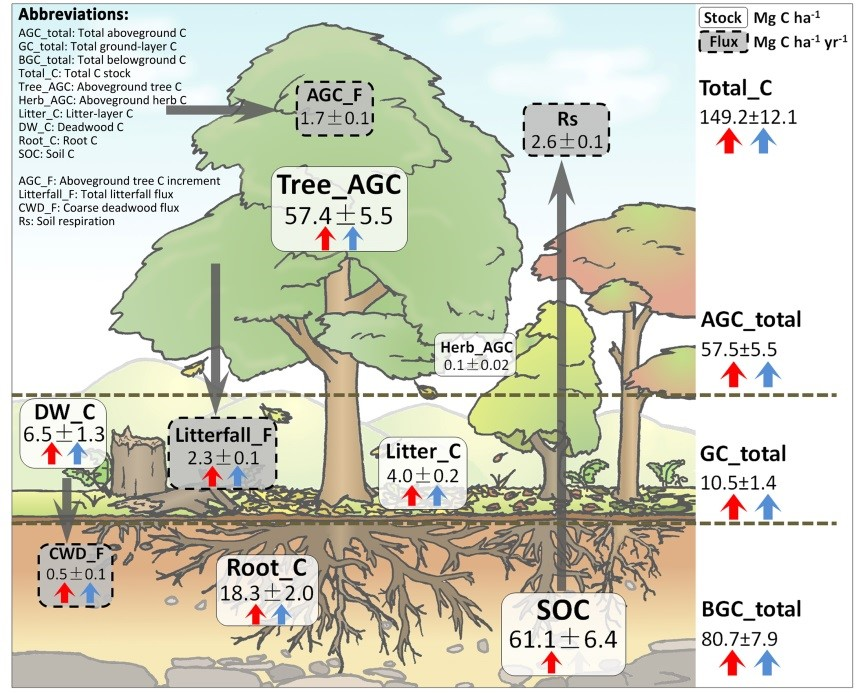
\includegraphics[width=13cm]{figs/carbon_cycle.jpg}
    \caption{Forest carbon cycle.}
    \label{fig:my_label}
\end{figure}

\subsection{Our work}
First, we developed a carbon sequestration model using the biomass method. We decomposed the objectives into two parts: carbon sequestration by forest products and carbon sequestration by forests. Management options (including cutting strategy and product strategy) were introduced into the model as an intermediate link between the two. 

We derived the best calculation function for forest biomass by curve fitting, and converted biomass into carbon sequestration based on relevant research. Forest products are broadly classified into three types of raw materials using cluster analysis for forest product carbon sequestration calculation. Combining the final destinations of trees and forest products (death, landfill and incineration), the amount of forest carbon sequestration was calculated. By analyzing the changes in carbon sequestration under different management scenarios, we can derive the amount of forest carbon sequestration under specified scenarios for reference of forest management measures.
The specific model is shown in Figure 2.(Task1)

Next, we use the entropy weight method to make a comprehensive evaluation of forest values. Combining carbon sequestration models and related research bases, indicators are constructed from three traditional dimensions of ecology, society and economy to reflect the comprehensive value of forests. We also introduce sustainability variables as a reference for forest development potential, taking into account the current green development trend.
The specific model is shown in Figure 3.(Task2)

Thirdly, we take a planted test forest in Qingping state-owned forest in Hunan Province as an example and substitute it into the model to study the best management plan. A 2 × 9 management plan matrix was obtained by setting different cutting rates and different product management strategies. We use the maximum value of the weighted sum of the factors as the objective function and program MATLAB to implement the model solution to obtain the best management plan under comprehensive evaluation.

Based on the existing management plan of this forest, we calculated the amount of carbon sequestered in the current forest over a 100-year period. Comparing the best management strategy and the existing management strategy, the transition plan of the two scenarios is derived. (Task3)

Finally, we performed a sensitivity analysis of the model with the results of the example calculations and explained and analyzed the strengths and limitations of the model. The results of the study are finally presented to the public in the form of a short non-technical article. We explain the design logic of the model in relatively easy-to-understand language to justify the forest management measures derived from the model that contradict conventional wisdom. The article \emph {More logging, more fixed carbon? Reasonable!} is presented.(Task4)




%Assumptions and Notations
%! TEX root = ./main.tex

\section{Assumptions and Notations}
\subsection{Assumptions}
%模型的假设条件,需要给出合理的解释(即为什么这样假设),可以用列表的形式
To simplify the problem and make it convenient for us to simulate real-life conditions, we make the following basic assumptions, each. Of which is properly justified.
\begin{itemize}
\item \textbf {We ignore soil carbon sequestration to simplify the model. }We believe that the ultimate purpose of the model is to provide a strategic reference for actual forest management managers, so introducing the variable of soil carbon sequestration, which has high indicator measurement cost and little correlation with forest management practices, is not necessary.
\item \textbf {We use the biomass method to determine the amount of carbon sequestered by trees and forest products.  }The biomass indicators are the most direct and accurate way to measure the amount of carbon sequestered by trees. The traditional growth environment indicators such as climate and geography, which are difficult to quantify, will be directly reflected in the growth of trees, and the data are easily available, making the model more concise and practical.
  \begin{itemize}
  \item We assume a constant ratio between volume and carbon sequestration for the same tree species.
  \item Total carbon sequestration in an S-shaped curve.
  \item We divided the total modeled carbon sequestration into two components: the trees themselves and the forest products. The amount of carbon sequestered by forest products is converted to the wood rate of different tree species.
  \end{itemize}
\item \textbf {We introduce changes in carbon sequestration from forest tree mortality and forest product waste.   }Not only the carbon sequestration during the tree growth period and the service life of forest products are considered, so that the model has the reference significance of the whole process.
\begin{itemize}
  \item We assume a constant tree mortality rate in the same forest and ignore the effects of chance factors such as fire.
  \item Only two categories of forest products treatment methods are considered: incineration and landfill. Landfill rate is calculated according to domestic waste treatment
  \end{itemize}
\item \textbf {The growth conditions of trees remain consistent in the forest.   }This may not be accurate due to different geographical factors including slopes, soil profiles, and water conditions. But the same climate and topographic feature guaranteed that the error of tree growth is small. Therefore, we use the average number to represent the same tree species in the forest.
\item \textbf {We take trees of the same species and same age as a whole, which is called "a cohort".} Based on the above assumptions, the trees ...
\end{itemize}


\newpage %为了格式整齐,暂时在这里翻一页。最后可以删掉换页命令。
\subsection{Notations}
%模型的变量表

The symbols we use in this paper are listed in the following Table 1.

% \usepackage{colortbl}
\begin{table}[ht] %当表格能够接在上一行之后,并完整地出现在同一页时,格式就不会乱。
\centering
\caption{Symbols used in this paper}
\begin{tabular}{ll}
\hline
\textbf{Symbols} & \textbf{Definition}                                          \\ 
\hline
    $BM_{ij}$   & Biomass of tree species $i$ at the age of $j$ years \\
    $H_{ij}$    & Height of tree species $i$ at the age of $j$ years \\
    $D_{ij}$    & Diameter at breast-height (DBH) of tree species $i$ at the age of $j$ years \\
    $\mu_{i}, \eta_{i}$   & Biomass proportion of trunk (with bark) and branches in trees of species $i$ \\
    $\rho_{i}$  & Density of the trunk of species $i$ \\
    $m_{i}$     & Tree mortality of species $i$ \\
    $N_{i}$     & Total amount of trees in species $i$ \\
    $n_{ij}(t)$ & The number of $i$ trees at the age of $j$ \\
\hline
    $P_{i}$     & Rotational felling period of $i$ species, after which trees would be cut \\
    $p_{i}$     & Tree felling rate \\
    $H_i(t)$    & The $t$th year biomass of felled trees in species $i$ \\
    $\alpha_i,\beta_i,\gamma_i$  & \makecell[l]{Proportion for sawn-wood, pulpwood and slash respectively in cut\\ down trees of $i$ species} \\
    $L_i$       & Service life of product $i$ \\
    $q$         & Landfill rate of forest products \\
    $r$         & Decomposition rate of forest products after landfill \\
\hline
    $K_{C}$     & Conversion coefficient from biomass to carbon sequestration \\
    $C(t)$      & Total carbon sequestration in the $t$th year\\
    $CT_{ij}(t)$& The $t$th year forest carbon sequestration of tree species $i$ at the age of $j$ \\
    $CP_{i}(t)$& The $t$th year product carbon sequestration of tree species $i$ \\
\hline
    $Pr_i$      & Price of product $i$ \\
    $EV(t)$     & Economic value of forest products in the $t$th year \\
    $x_{ij}$    & Score of the $j$th strategy under indicator $i$ \\
    $norx_{ij}$ & Normalized score $x_{ij}$\\
    $Y_{ij}$    & Proportion of $norx_{ij}$ in all $norx_{i}$s \\
    $E_{i}$     & Information entropy of indicator $i$ \\
    $W_{i}$     & The weight of indicator $i$\\
    $S_{j}$     & Final score for forest value under $j$th strategy. \\
\hline
\end{tabular}
\end{table}

%综合评价模型写完之后可能还有一些变量需要添加。

%Explain the model in task I
%! TEX root = ./main.tex

\section{The Model of Carbon Sequestration}
%模型图
The carbon sequestration model can be summarized in in Figure 2.

\begin{figure}[htp]
    \centering
    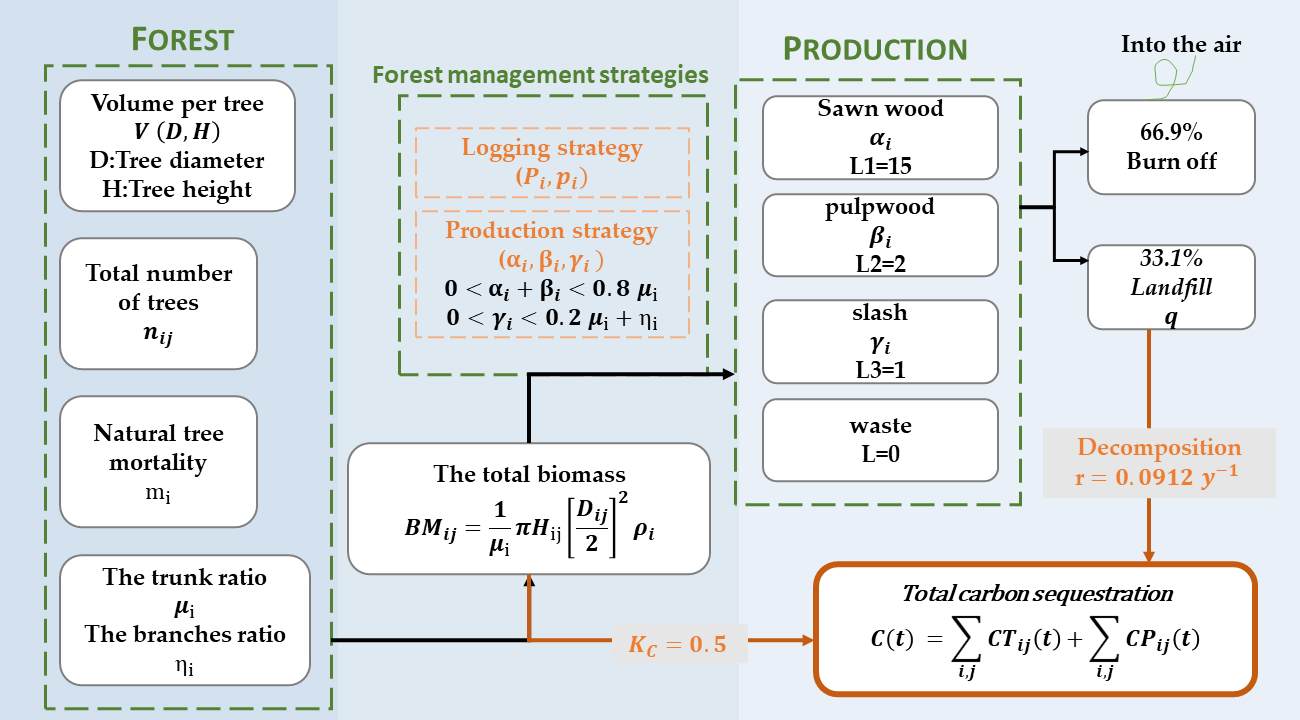
\includegraphics[width=15cm]{figs/Carbon_model.png}
    \caption{Carbon sequestration model.}
    \label{fig:my_label}
\end{figure}

\subsection{Input}

\subsubsection{Biomass function}
Based on the underlying assumptions, we calculate the amount of carbon sequestration by converting the volume of trees into biomass. To calculate the biomass $BM_{ij}$, we first calculated the biomass of the trunk according to the diameter (at breast-height), height and density of the tree, and then calculated the total biomass according to the biomass proportion of the trunk in an individual plant.
\begin{eqnarray}
B M_{i j} & = & \frac{1}{\mu_{i}} \pi H_{i j}\left[\frac{D_{i j}}{2}\right]^{2} \rho_{i}
\end{eqnarray}

It is required that the annual variation data of DBH and height be be collected. The data are used to fit the variation function of tree DBH and tree height, $D_{ij}$ and $H_{ij}$, where $i$ stands for species and $j$ stands for the age. Several S-shaped functions are used for fitting, from which the ones with the best fitting are chosen to represent the variation:
\begin{equation}
\begin{aligned}
    Y&=Kt^{b},\\
    Y&=\frac{t}{a+b t},\\
    Y&=\frac{K}{1+a e^{-bt}},\\
    Y&=K a^{b t},\\
\end{aligned}
\end{equation}
where $K,a,b$ are undetermined constants. With diameter and height functions obtained, the biomass is calculated via formula (1).

\subsubsection{Tree age distribution and tree mortality}
Assuming that the mortality $m_i$ of each species is constant and the total number of trees remains $N_i$, the number of trees of different ages in the current forest can be calculated as follows.
Mark the planting time of the artificial forestation as $T_i$ years ago ($t=-T_i$. Each year, a proportion of $m_i$ was eliminated due to natural death. Dead trees were replaced by new-born trees, controlling the total number to $N_i$. The numbers of trees at $t=0$ are listed below.

\begin{equation}
\begin{array}{c}
n_{i, T_{i}} = N_{i}\left(1-m_{i}\right)^{T_{i}-1} \\
n_{i j} = N_{i} m_{i}\left(i-m_{i}\right)^{j-1}, j = 2,3, \ldots, T_{i}-1 \\
n_{i 1} = N_{i} m_{i}
\end{array}
\end{equation}

Given the average diameter $\overline{D_{i}}$  of each tree species, the natural mortality $m_i$ of trees under the environmental conditions can be obtained by bisection method. And by applying $m_i$, the age distribution of trees at $t=0$ can be obtained using formula (3).

\begin{equation}
\overline{D_{i}}=\frac{\sum_{j=1}^{T_{i}} D_{i j} n_{i j}}{\sum_{j=1}^{T_{i}} n_{i j}}
\end{equation}

\subsubsection{Coefficient of biomass conversion to carbon sequestration}
Forest carbon sequestration is mainly calculated by measuring the biomass of forest vegetation and multiplying it by the biomass - carbon conversion coefficient $K_c$. The 2006 IPCC Guidelines for National GHG Inventories recommended the carbon ratio of aboveground forest biomass. 

To simplify the model, we take $K_c$ as 0.5, which is the average value of empirical data given by IPCC.


\subsubsection{Service life of the product}

Based on the nature of the wood used, we classify forest products into sawn-wood, pulp-wood and slash.The specific definition is as follows.

% \usepackage{colortbl}
\begin{table}[htp]
\caption{Classification of forest products.}
\begin{tabular}{llll} 
\hline
\textbf{Product} & \textbf{Instance}               & \textbf{Service life /year} & \textbf{Disposal mode}                                                                                          \\ 
\hline
sawn-wood        & Furniture,
  building materials & 15                          & Landfill or incineration.                                                   \\
pulp-wood        & Plywood,
  cardboard, paper     & 10~                         & Landfill or incineration. \\
Slash            & Fuel                            & 1                           & Burned.                                                                                                         \\
\hline
\end{tabular}
\end{table}

The average product life $L_1$ of Sawn-wood is assumed to be 15 years, the life $L_2$ of pulp-wood is assumed to be 10 years, and the life $L_3$ of slash is assumed to be 1 year. The discarded part has no service life and is not included in the calculation system.

\subsubsection{Landfill and decomposition parameters}
We divided the final destination of forest products into landfill and incineration. Any treatment other than landfill is treated as incineration, which releases CO$_2$ directly into the air and does not count in the carbon sequestration system.

According to the \emph{2020 Annual Report on The Prevention and Control of Environmental Pollution by Large and medium-sized Cities} released by the Ministry of Ecology and Environment of China, the current landfill rate $q$ in China is 33.1\%, and the decomposition rate $r$ is 0.0912 per year\cite{Decomposition_rate}. The carbon sequestration effect of these forest products is included in the calculation system.

\subsection{Calculation carbon sequestration}
\subsubsection{Variation of age distribution}
The tree age distribution of each year from $t=0$ is obtained by iteration. The relationship between the age distribution of trees in the two adjacent years is

\begin{equation}
\begin{aligned}
    n_{i1}(t+1)&=N_i m_i + \sum_{j>P_i}n_{i j}\times(1-m_i)\timesp_i \\
    n_{i j}(t+1)&=n_{i j}(t)\times(1-m_i),1<j<P_i\\
    n_{i j}(t+1)&=n_{i j}(t)\times(1-m_i)\times(1-p_i),j\ge P_i\\
\end{aligned}
\end{equation}

Formula (5) means that trees that were dead or cut down would be replaced by new-born trees in the next year.

\subsubsection{Carbon sequestration in trees}

The carbon sequestration in trees can be converted from biomass of living trees.

\begin{equation}
    CT_i(t) = K_C\times \sum_{j}BM_ij\times n_{ij}(t)
\end{equation}

\subsubsection{Carbon sequestration in products}
For each year, the biomass of cut-down trees in species $i$ is
\begin{equation}
    H_i(t)=\sum_{j>P_i}n_{ij}(t)\times p_i\timesBM_{ij}
\end{equation}
The biomass percentage of trees that are made into sawn-wood, pulpwood and slash are respectively $\alpha_i,\beta_i,\gamma_i$, their service lives being $L_1,L_2,L_3$. A proportion of $q$ for sawn-wood and pulpwood ends up in landfill. The decomposing rate in landfill is $r$. Therefore, the carbon sequestration in products and its wastes comply with the following relationship:

\begin{equation}
\begin{aligned}
    \frac{CP_i(t)}{K_C}=&\sum_{\Delta t=0}^{L_1}H_i(t-\Delta t)\times \alpha_i+\sum_{\Delta t=0}^{L_2}H_i(t-\Delta t)\times \beta_i+\sum_{\Delta t=0}^{L_3}H_i(t-\Delta t)\times \gamma_i\\
    &+\sum_{\Delta t=L_1}^{\infty}H_i(t-\Delta t)\times \alpha_i\times e^{-r(\Delta t-L_1)}+\sum_{\Delta t=L_2}^{\infty}H_i(t-\Delta t)\times \beta_i\times e^{-r(\Delta t-L_2)}
\end{aligned}
\end{equation}

\subsection{Management strategies}
\subsubsection{Logging strategy}
Logging strategy is an important part of forest management strategy, which directly affects the balance between forest and forest products. We introduce a logging strategy (p$_i$,P$_i$). This means that for every tree species $i$, a proportion equal to $p_{i}$ of trees should be cut down for trees older than the age of rotation period $P_i$.

By default, $p_i$ varies continuously between 0 and 1. For simplicity, we set $p_i$  to the same for each tree species.

Based on actual forest farm data, we tested the changes in carbon sequestration resulting from different logging strategies.

\subsubsection{Production strategy}
Forest products are divided into three categories according to their wood properties -- sawn-wood, pulp-wood and slash. They are represented by $\alpha_i$, $\beta_i$ and $\gamma_i$ respectively. Product strategies can be described by number pairs ($\alpha_i$, $\beta_i$, $\gamma_i$). The waste in the production process is treated as a product with a life cycle of 0, which means rapid and complete decomposition within a year.

The biomass of the trunk of the whole tree is $\mu_i$, and the biomass of the branches is $\eta_i$. Assuming 80\% of the trunk can be made into sawn-wood, the rest of the trunk and branches can be made into pulpwood or slash. Everything else was discarded. We derive the following inequality to generalize the state of production.
\begin{equation}
\begin{array}{c}
0<\alpha_{i}+\beta_{i}<0.8 \mu_{i} \\
0<\gamma_{i}< \mu_{i}+\eta_{i} \\
\end{array}
\end{equation}

To simplify the model, the production strategy takes two extremes:

1.$\left(\alpha_{i}, \beta_{i}, \gamma_{i}\right)=\left(0.8 \mu_{i}, 0.2 \mu_{i}+\eta_{i}, 0\right)$

2.$\left(\alpha_{i}, \beta_{i}, \gamma_{i}\right)=\left(0, \mu_{i}, \eta_{i}\right)$

The former is the most conducive to carbon sequestration distribution, that is, to achieve the longest life of the product. The latter is the most unfavorable to carbon sequestration. Any other situation should be in between the two.

\subsection{Output}
In the above carbon sequestration model, carbon sequestration is divided into forest carbon sequestration and forest product carbon sequestration. The parameters can be used to calculate the carbon sequestration of each forest by fitting the actual forest farm data.
\begin{equation}
\begin{array}{c}

C(t)=\sum_{i,j}CT_{i}(t)+\sum_{i}CP_{i}(t)

\end{array}
\end{equation}

%Explain the model in task II
%! TEX root = ./main.tex

\section{Multi-aspect Decision Model of Forest Management}


\begin{figure}[htp]
    \centering
    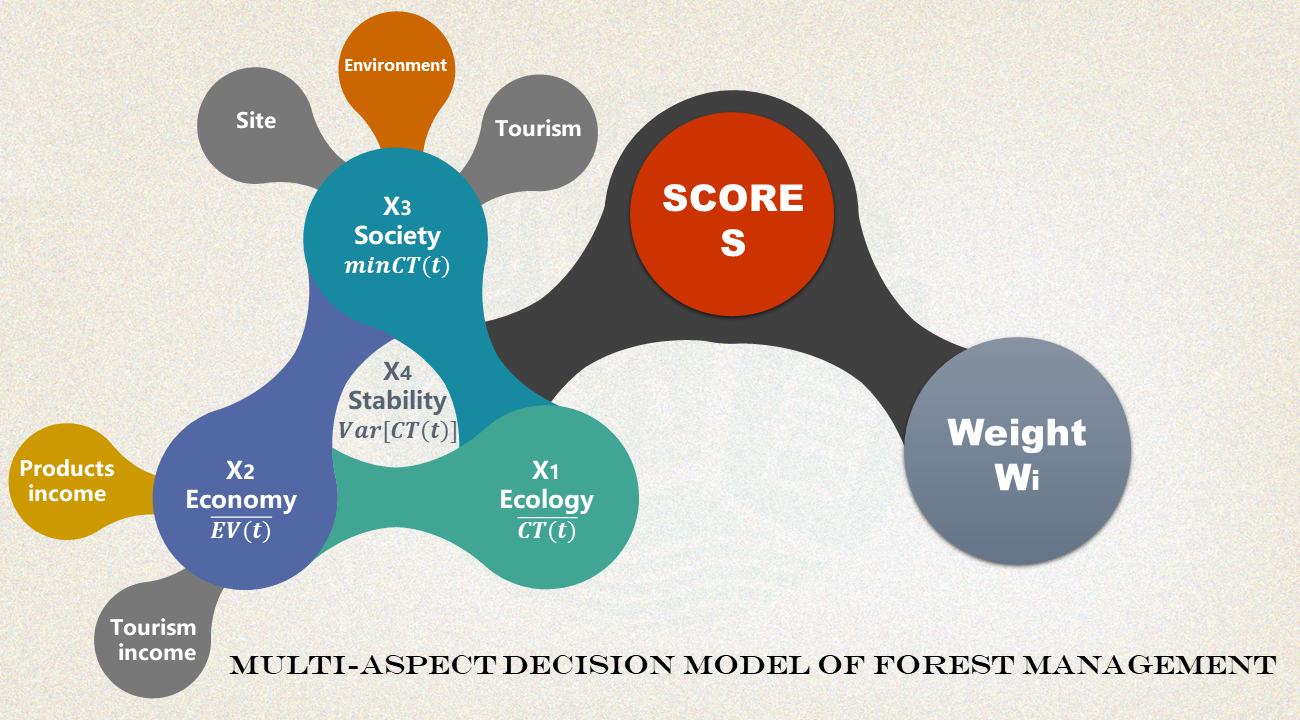
\includegraphics[width=15cm]{figs/multi_model.png}
    \caption{Multi-aspect Decision Model of Forest Management.}
    \label{fig:my_label}
\end{figure}

Based on the definition of forest value\cite{multi_system}, this paper establishes indicators from three traditional dimensions of ecology, society and economy to reflect the comprehensive value of forest based on certain principles, and introduces sustainability variables as references for forest development potential. Finally, the level of ecological, economic and social development of forest system was classified and comprehensively evaluated by entropy weight method. According to the evaluation results of specific forests, the model can provide suggestions for forest management.

The Multi-aspect Decision Model of Forest Management can be summarized in in Figure 3.

\subsection{Evaluation dimensions of forest value}

\subsubsection{Ecological value}
"Canopy density" is considered as a classic index reflecting the ecological value of a forest, which can be used to measure the thickness of a forest. However, the forest data directly reflecting canopy density is difficult to obtain in reality. Through correlation analysis, we can conclude that canopy density is positively correlated with leaf biomass, so variables directly related to biomass can be used as proxy variables.

In the carbon sequestration model, we have concluded that the amount of biological carbon sequestration $CT(t)$is proportional to the biomass, so it can reflect the growth degree of the forest. The greater the biomass, the more mature the forest and the higher its ecological value. Therefore, we derive the following formula to quantitatively calculate forest ecological value.

Considering the long duration of the ecological effect of the forest, we take the average value of carbon sequestration for 100 years as the ecological indicator.

$$
x_1=\overline{CT(t)}
$$


\subsubsection{Economic value}
From the perspective of benefit measurement and ecological compensation, forest economic value is often used as the economic benefit of forest, that is, the monetary expression of forest value in the commodity society. In the process of maintaining the biological characteristics of the forest, the forest products or ecological environment generated in the forest ecosystem and its influence range can be used by people. The monetary expression in the commodity economy is the value of forest economic benefits, which is also called the total economic value of the forest.
%计算过程%

The calculation process of economic value of forest products is as follows:

Sawn-wood       :   $Pr_1$=2300 yuan/cubic meter

Pulp-wood       :   $Pr_2$=5300 yuan/cubic meter

Slash           :   $Pr_3$=900 yuan/ton

$$EV(t)=\sum_{i}H_i(t)\times(\alpha_iPr_{1}+\beta_i Pr_{2}+\gamma_iPr_{3})$$

Finally, take the 100-year average of returns as an economic indicator.

$$x_2=\overline{EV(t)}$$

In the article, the economic value of forest ecosystems was not included in the evaluation of the economic value of forests for the following reasons.

\begin{itemize}
    \item The economic value of forest ecological environment is usually reflected as tourism resources. The development of forest tourism is usually influenced by cultural factors and local socio-economic development, while the change of ecological environment caused by forest management strategy has no significant impact on local socio-economic development.
    \item The marginal returns to the state of forest ecosystems are low. The high level of forest ecology has a small impact on economic returns. The economic benefits of ecological environment can basically only be qualitative but not quantitative.
\end{itemize}

Based on the above reasons, this part of the economic income is included in the social value evaluation dimension of the forest in the model rather than the economic value dimension.

\subsubsection{Social value}

Forest site selection, forest ecology, and the degree of tourism development are important influencing factors and reference indicators of the social value of forests.

In the perspective of forest ecology, we choose the minimum value of biomass as the variable. Forest biomass directly reflects the ecological condition and resource affluence of the forest, which can be regarded as the guaranteed part of the forest available for ecotourism and affects the social value of the forest.

The individual effects of forest site selection and degree of tourism development are significant, and the particular forest site location may play a decisive influence on forest management measures. For example, some forests serve as ecological reserves and are largely free of economic activity. For special cases a separate analysis of the forest site is required.

For conventional forest land, the discussion of forest site location and the degree of tourism development is not significant, and the model discards these two factors for the sake of simplifying the model.

$$
x_3=\min CT(t)
$$

Compared with the hierarchical analysis and fuzzy integrated judgment methods commonly used in social value evaluation, the choice of measurable biomass indicators to quantify the social value of forests can eliminate the subjectivity in value judgment. It is also more direct and objective in data acquisition, which enhances the universality of the model.

\subsubsection{Stability}

As the concept of green development is put forward, the evaluation of forest value should not be limited to the present ecological, economic and social value. In fact, ecological sustainability, economic sustainability and social sustainability are all important components of the evaluation of each dimension.

We need to integrate sustainability principles into forest management measures in order to grasp the potential and potential problems of sustainable development of forests and achieve the desired ecological, economic and social goals.

The stability of forest ecological condition directly reflects the sustainability of forest. We used the statistical variance of carbon sequestration to measure forest sustainability.

$$
x_4=\frac{\sum_{t=1}^{100}(CT(t)-\overline{CT})^2}{100-1}
$$




\subsection{Comprehensive evaluation process of multidimensional value}

The model has addressed the economic, social, ecological and sustainability dimensions of forest values respectively. In order to carry out comprehensive evaluation, we need to homogenize the indicators of each dimension, and give the comprehensive score of forest through entropy weight method, so as to evaluate and guide forest management measures. 

For each index, the values of $n$under different schemes are obtained and scaled to the range of [0,1].

$$
norx_{ij}=\frac{\max x-x}{\max x-\min x}
$$

Calculate the information entropy of each index $E_i$

$$
Y_{ij}=\frac{norx_{ij}}{\sum_{j=1}^n norx_{ij}}
$$
$$
E_i=-\frac{1}{\ln n}\sum_{j=1}^{n}Y_{ij}\ln Y_{ij}
$$

Find out the weight of each indicator $W_i$

$$
W_i=\frac{1-E_i}{4-\sum E_i}
$$

The final score $S$ of the management scheme is calculated as follows.

$$
S=\sum_{i=1}^4 W_i\times x_i'
$$

%待补充


%Implementation
%! TEX root = ./main.tex

\section{Implementation of Decision Model}

Next, we take a man-made experimental forest in Qingping National Forest Farm in Hunan province as an example(Figure 4). We substitute the forest data\cite{Hdata,TaiwaniaDensity,ToonaDensity} into the above model to investigate the best management strategies.

\begin{figure}[htp]
    \centering
    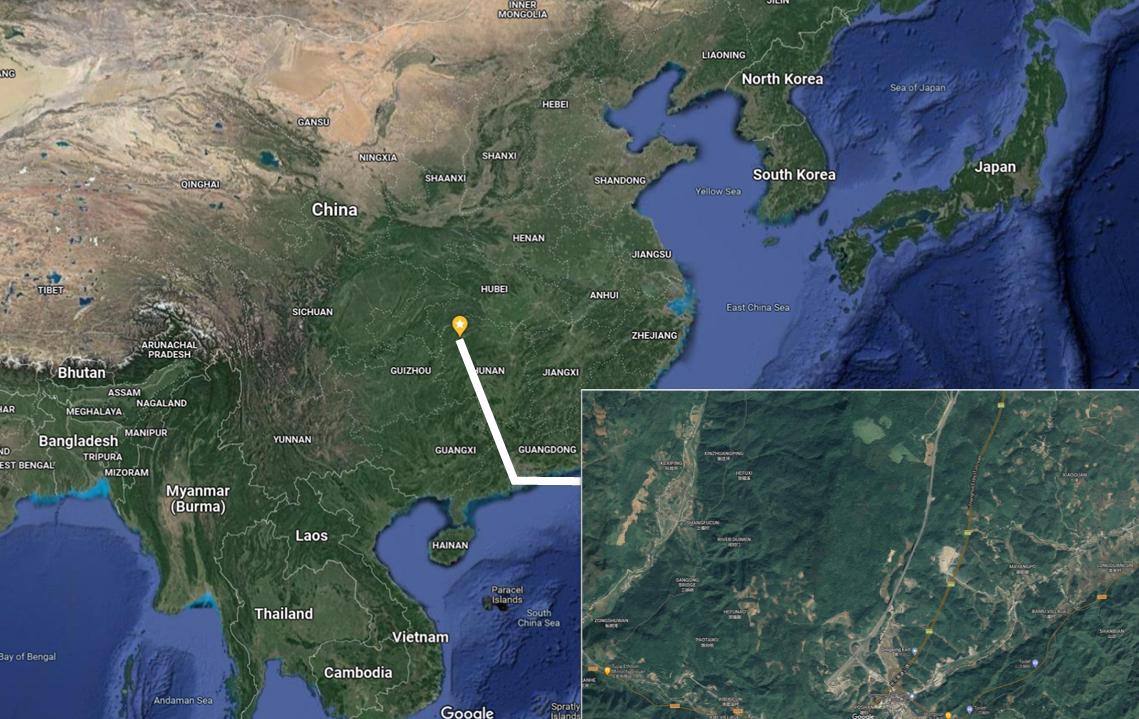
\includegraphics[width=15cm]{figs/map.png}
    \caption{Location of Qingping State-owned Forest Farm, Hunan Province, China.}
    \label{fig:my_label}
\end{figure}

\subsection{The matrix of management strategies}
By setting the 0 and 1 within the scope of different deforestation (0,0.01,0.02,0.03,0.05,0.1,0.3,0.5,1) and the different product management strategies (two extreme), get 2 x 9 matrix management plan. This strategy matrix will contain maximum and minimum values on each evaluation indicator.

We take the maximum value of the weighted sum of all factors as the objective function, realize the model solution through MATLAB programming, and get the best management  strategies. The specific process is as follows.

\subsection{Basic validation of the model}

First, We verified the relationship between total carbon sequestration and forest products and forest carbon sequestration:
$$
C(t)=\sum_{i,j}CT_{i,j}(t)+\sum_{i,j}CP_{i,j}(t)
$$

The specific case ($p_i$ =0.75, product strategy 1) is shown in figure 5. The curve relations in the other 28 cases are the same, which will not be shown in this paper.

\subsection{Management strategy}

\textbf{The management strategy} is divided into two parts: logging strategy and production strategy.

\subsubsection{Logging strategy}

Suppose the area of the three kinds of forest is 10hm$^2$. The total area of the forest farm is 30hm$^2$, and the sum of the three kinds of trees is known, that is, the southern jujube, Taiwan fir and Chinese toona. The oldest Chinese date is 35 years old, and Taiwan fir and Chinese toona are 40 years old (T$_i$). No logging is known to have taken place in these years. We get the following results:……

As a rule of thumb, we default $P_1$=25,$P_2$=50,$P_3$=38 (unit=year).

In terms of the choice of logging plan, we set different $p_i$ and obtained the curve of carbon sequestration as Figure $6$.
\begin{figure}[htbp]
\centering
\begin{minipage}[t]{0.48\textwidth}
\centering
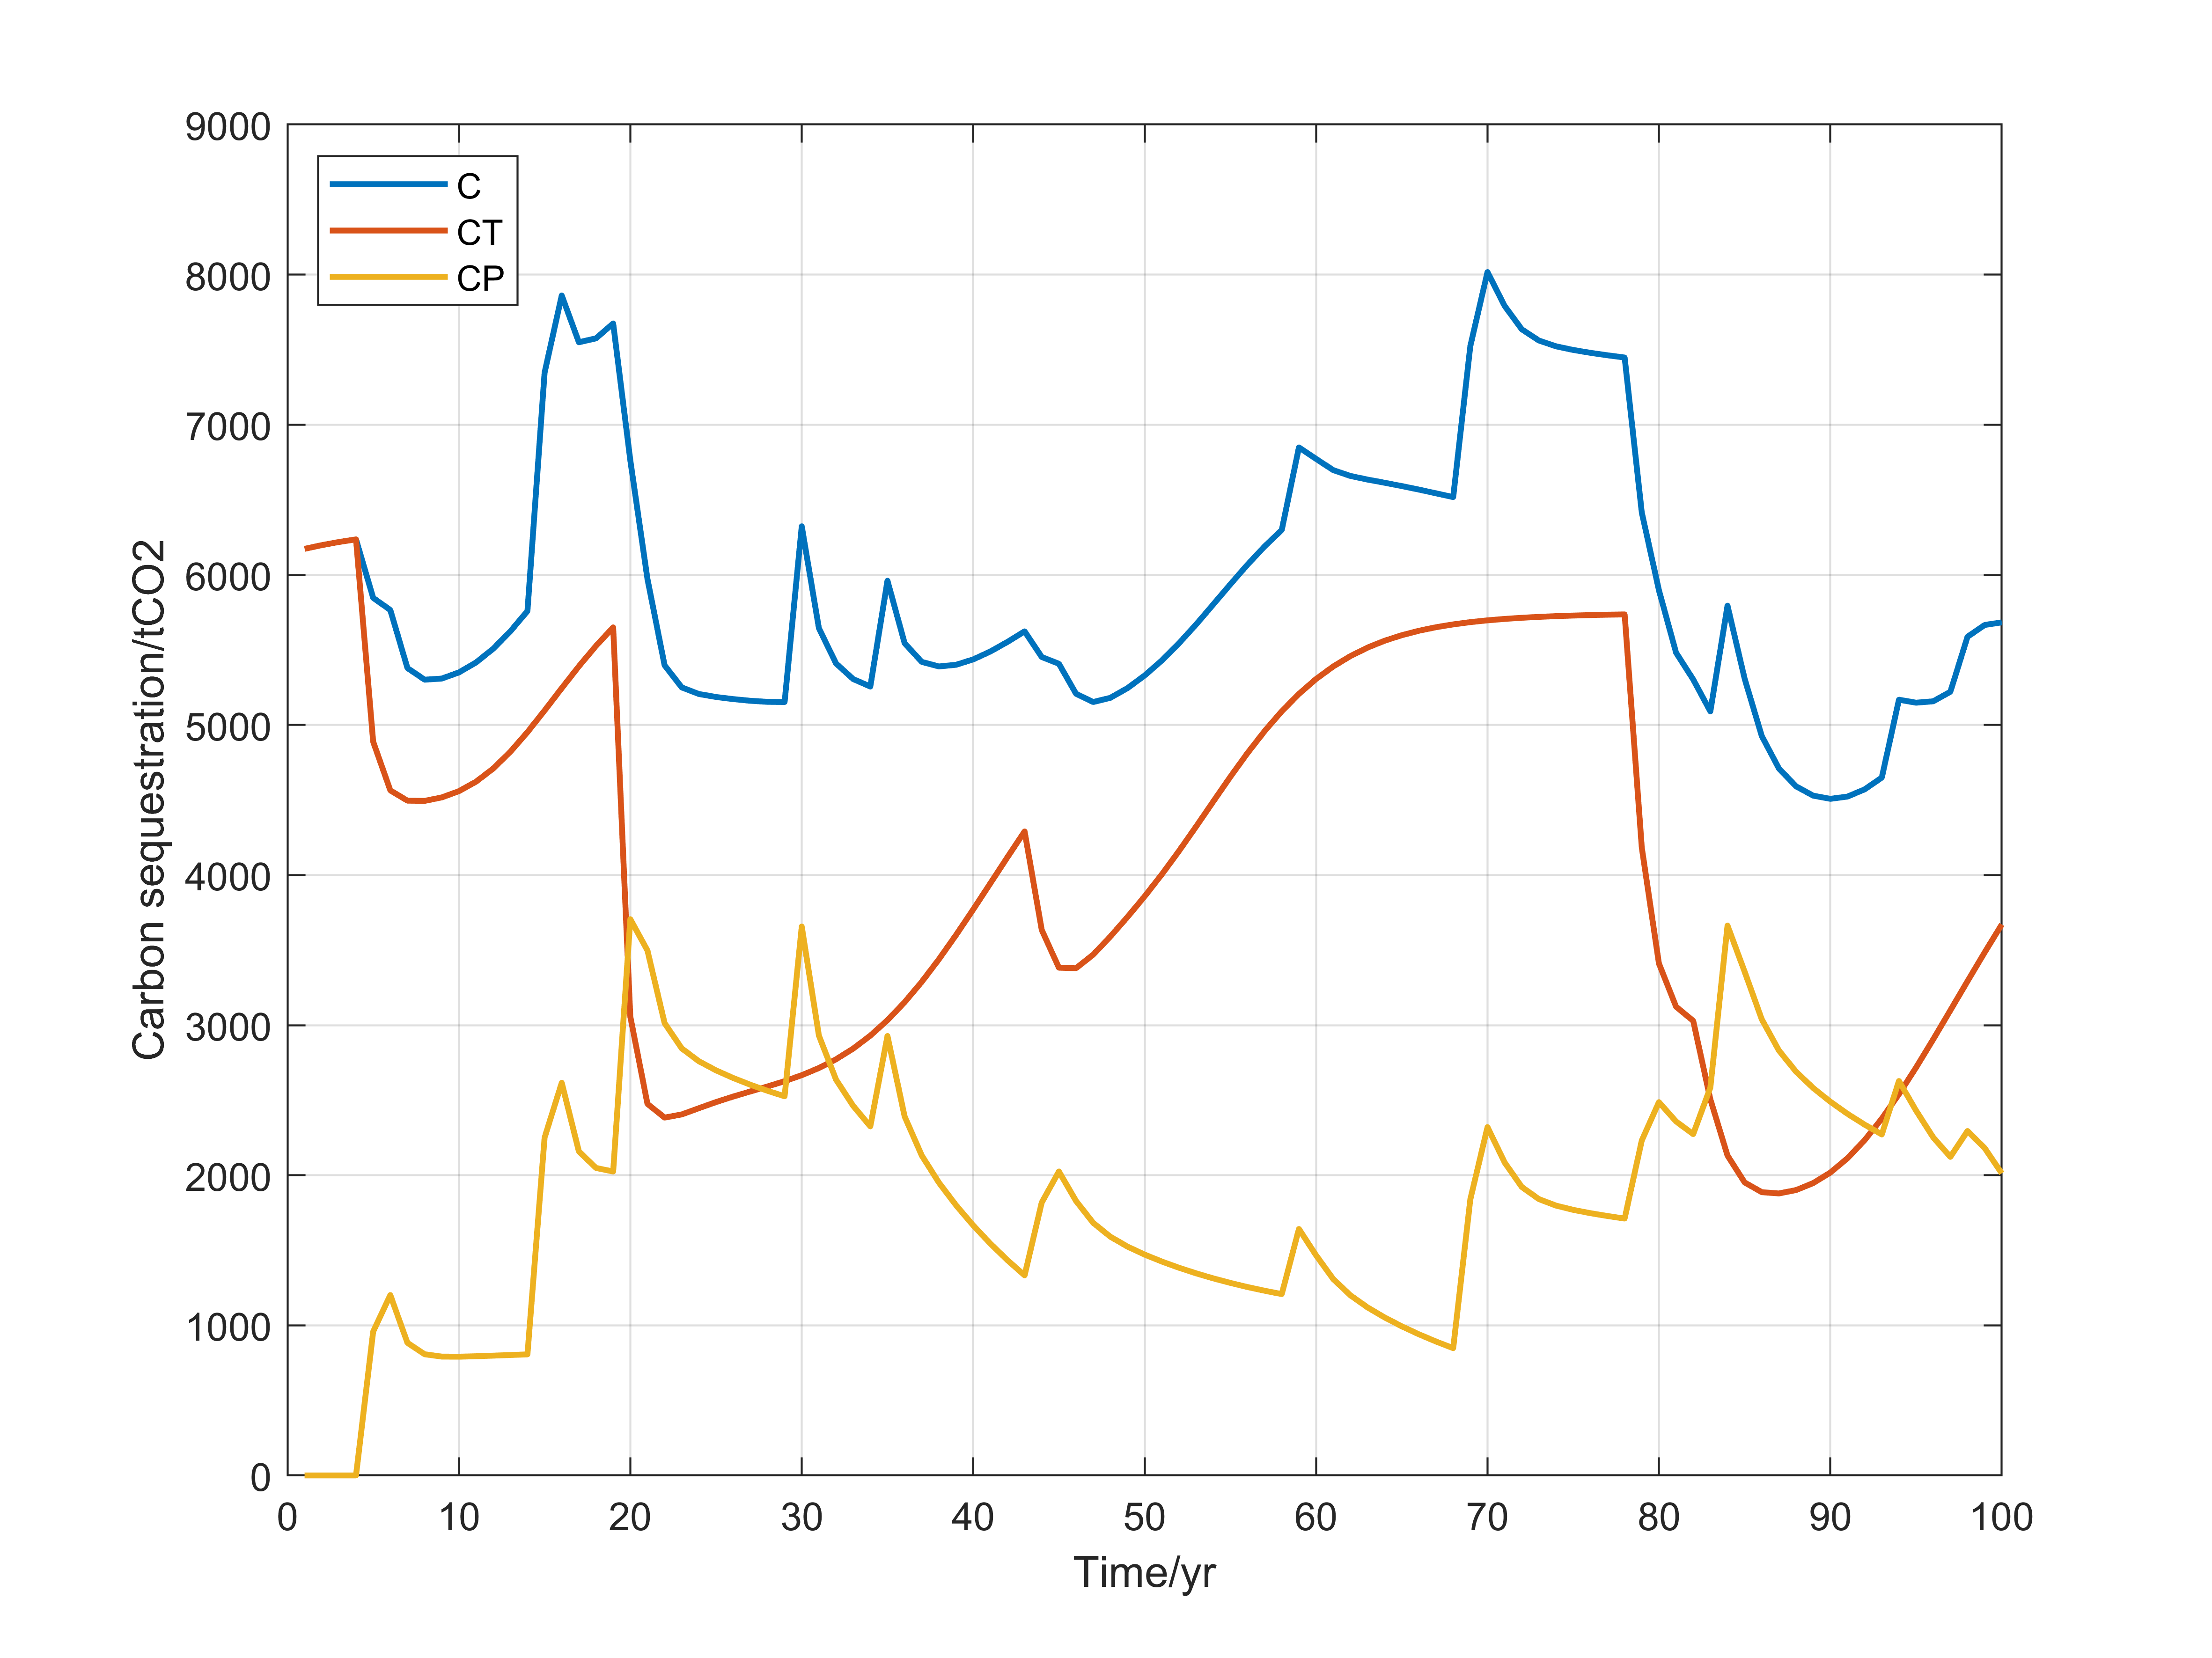
\includegraphics[width=6cm]{figs/CS.png}
\caption{Carbon sequestration under specific conditions.}
\end{minipage}
\begin{minipage}[t]{0.48\textwidth}
\centering
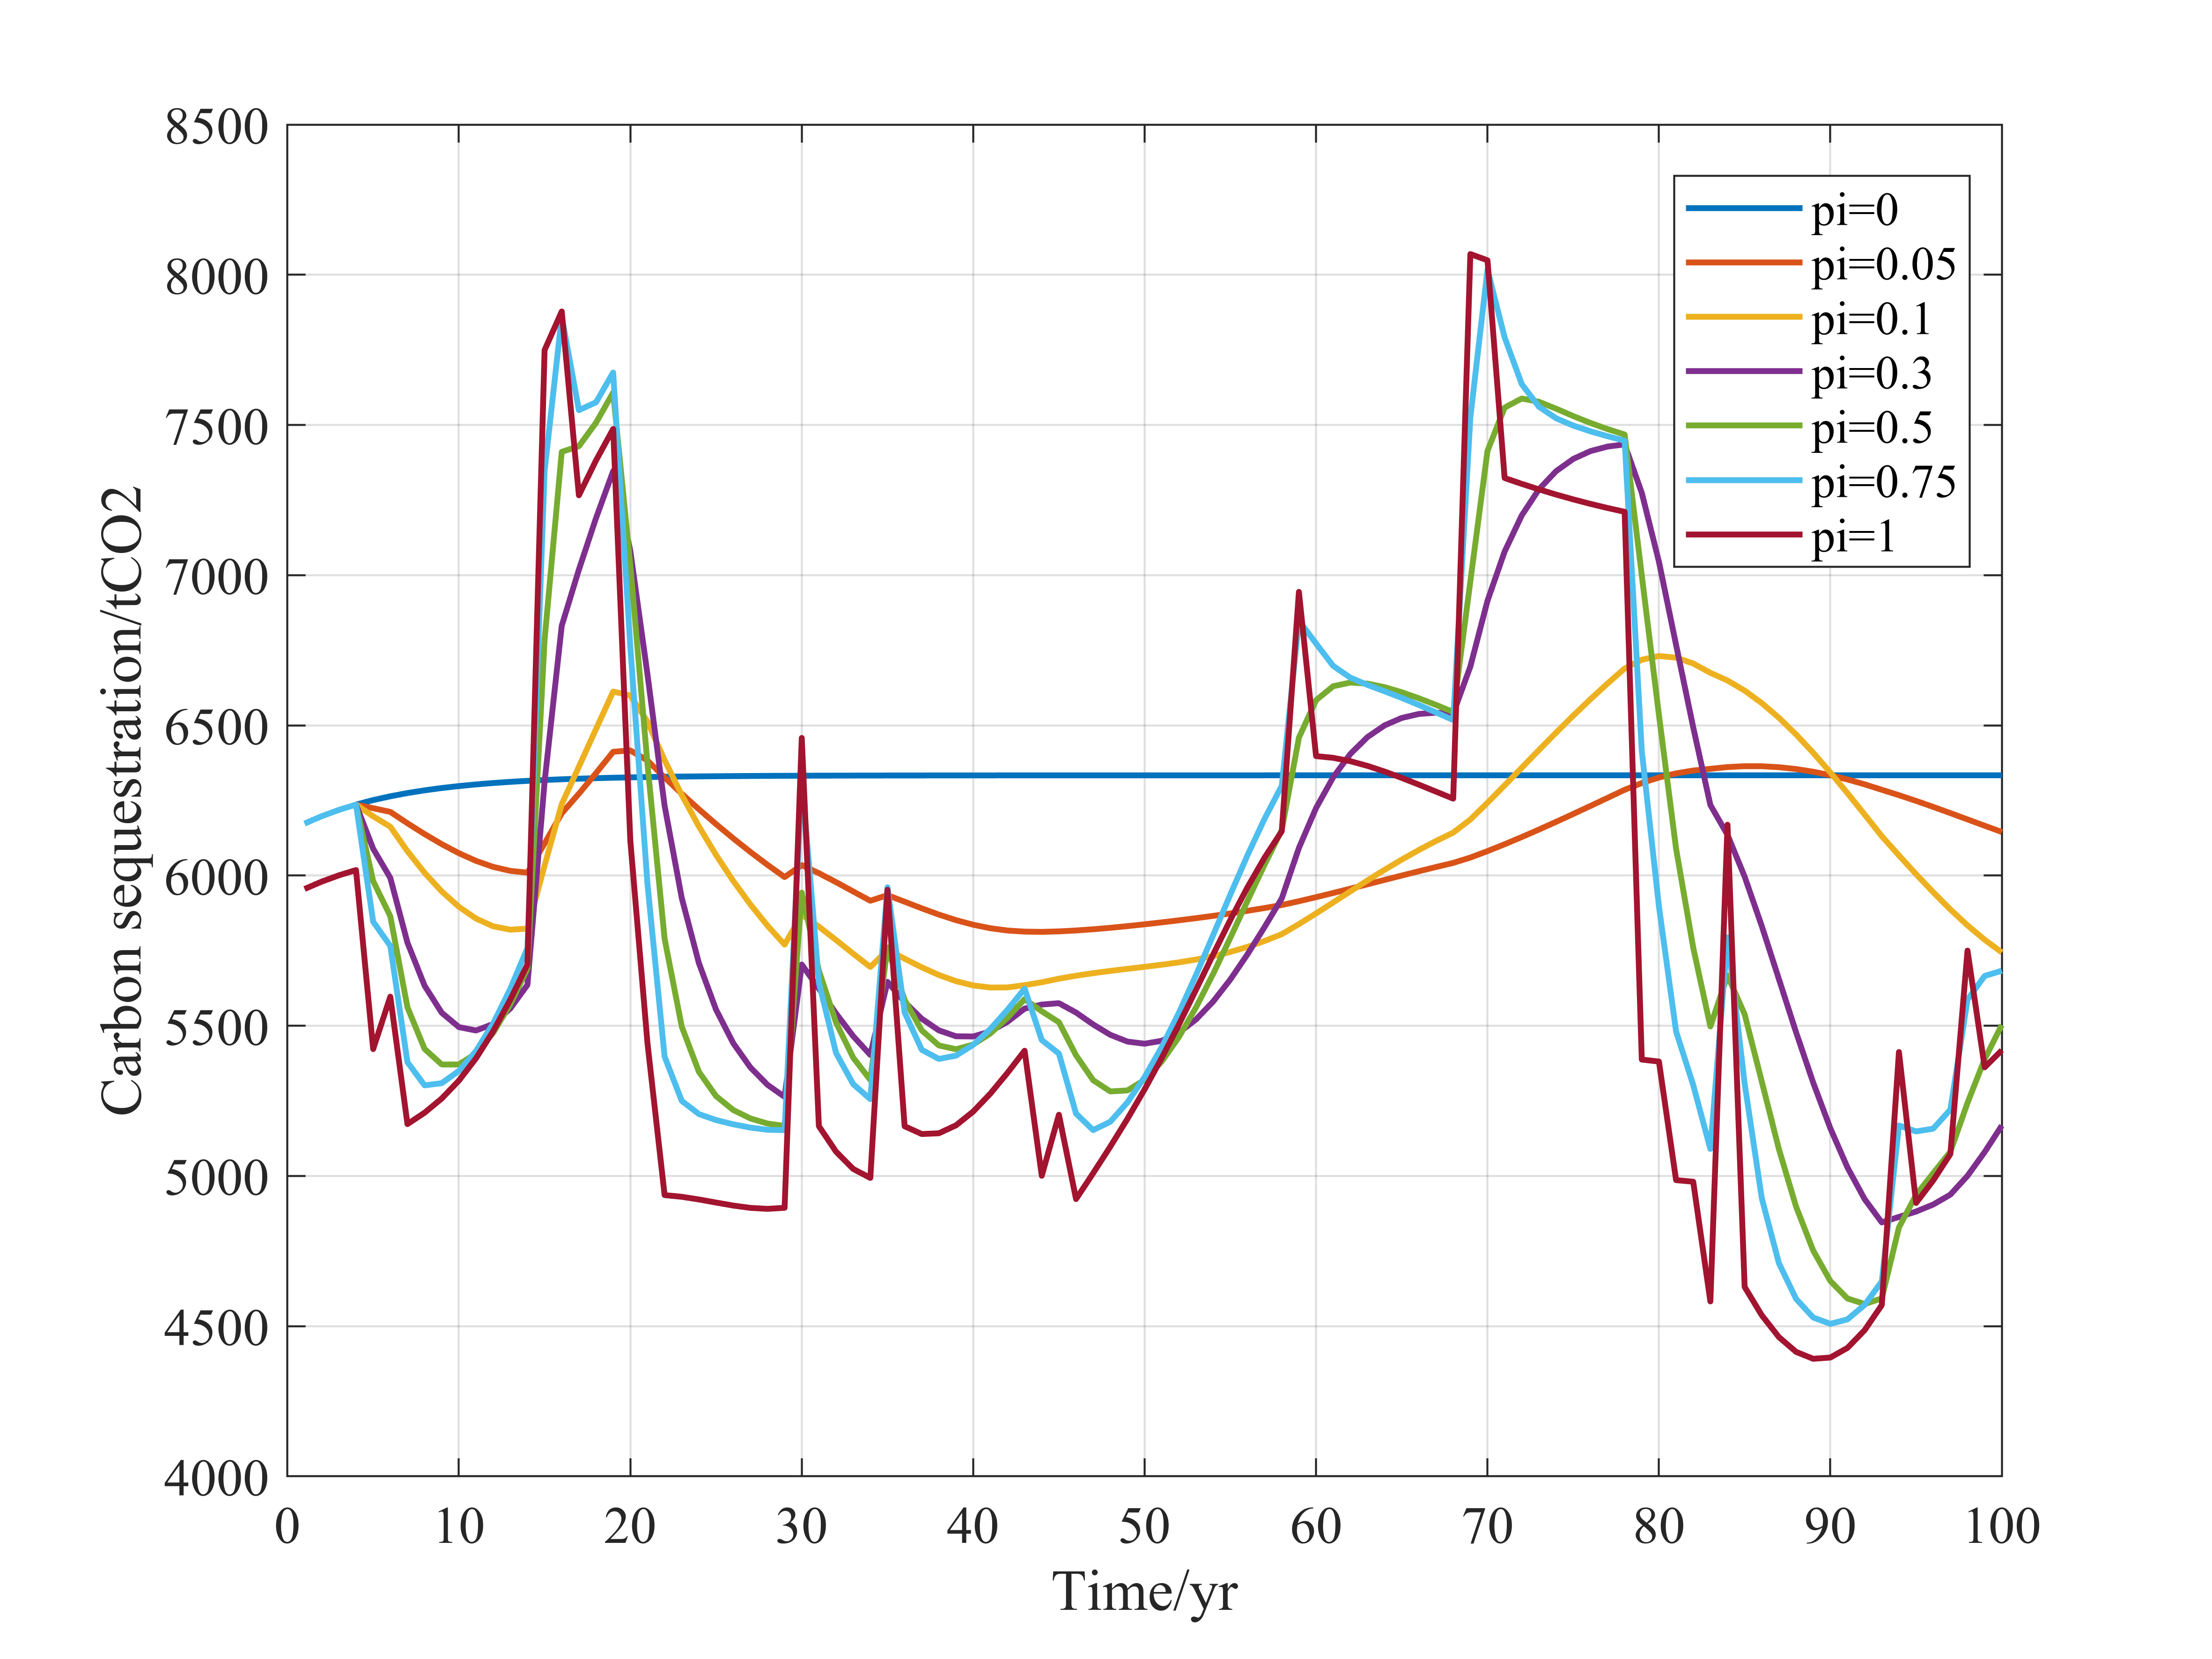
\includegraphics[width=6cm]{figs/pi_s.png}
\caption{Carbon sequestration performance of management strategies at different logging rates.}
\end{minipage}
\end{figure}

According to the results, higher carbon sequestration can be achieved when $p_i$ =0.01.

\subsubsection{Production strategy}

In terms of production strategy selection, we compared and calculated two extreme strategies:

1.$\left(\alpha_{i}, \beta_{i}, \gamma_{i}\right)=\left(0.8 \mu_{i}, 0.2 \mu_{i}+\eta_{i}, 0\right)$

2.$\left(\alpha_{i}, \beta_{i}, \gamma_{i}\right)=\left(0, \mu_{i}, \eta_{i}\right)$

As shown in Figure $7$, strategy 1 performs better in the model and can achieve higher carbon sequestration.
\begin{figure}[htbp]
\centering
\begin{minipage}[t]{0.48\textwidth}
\centering
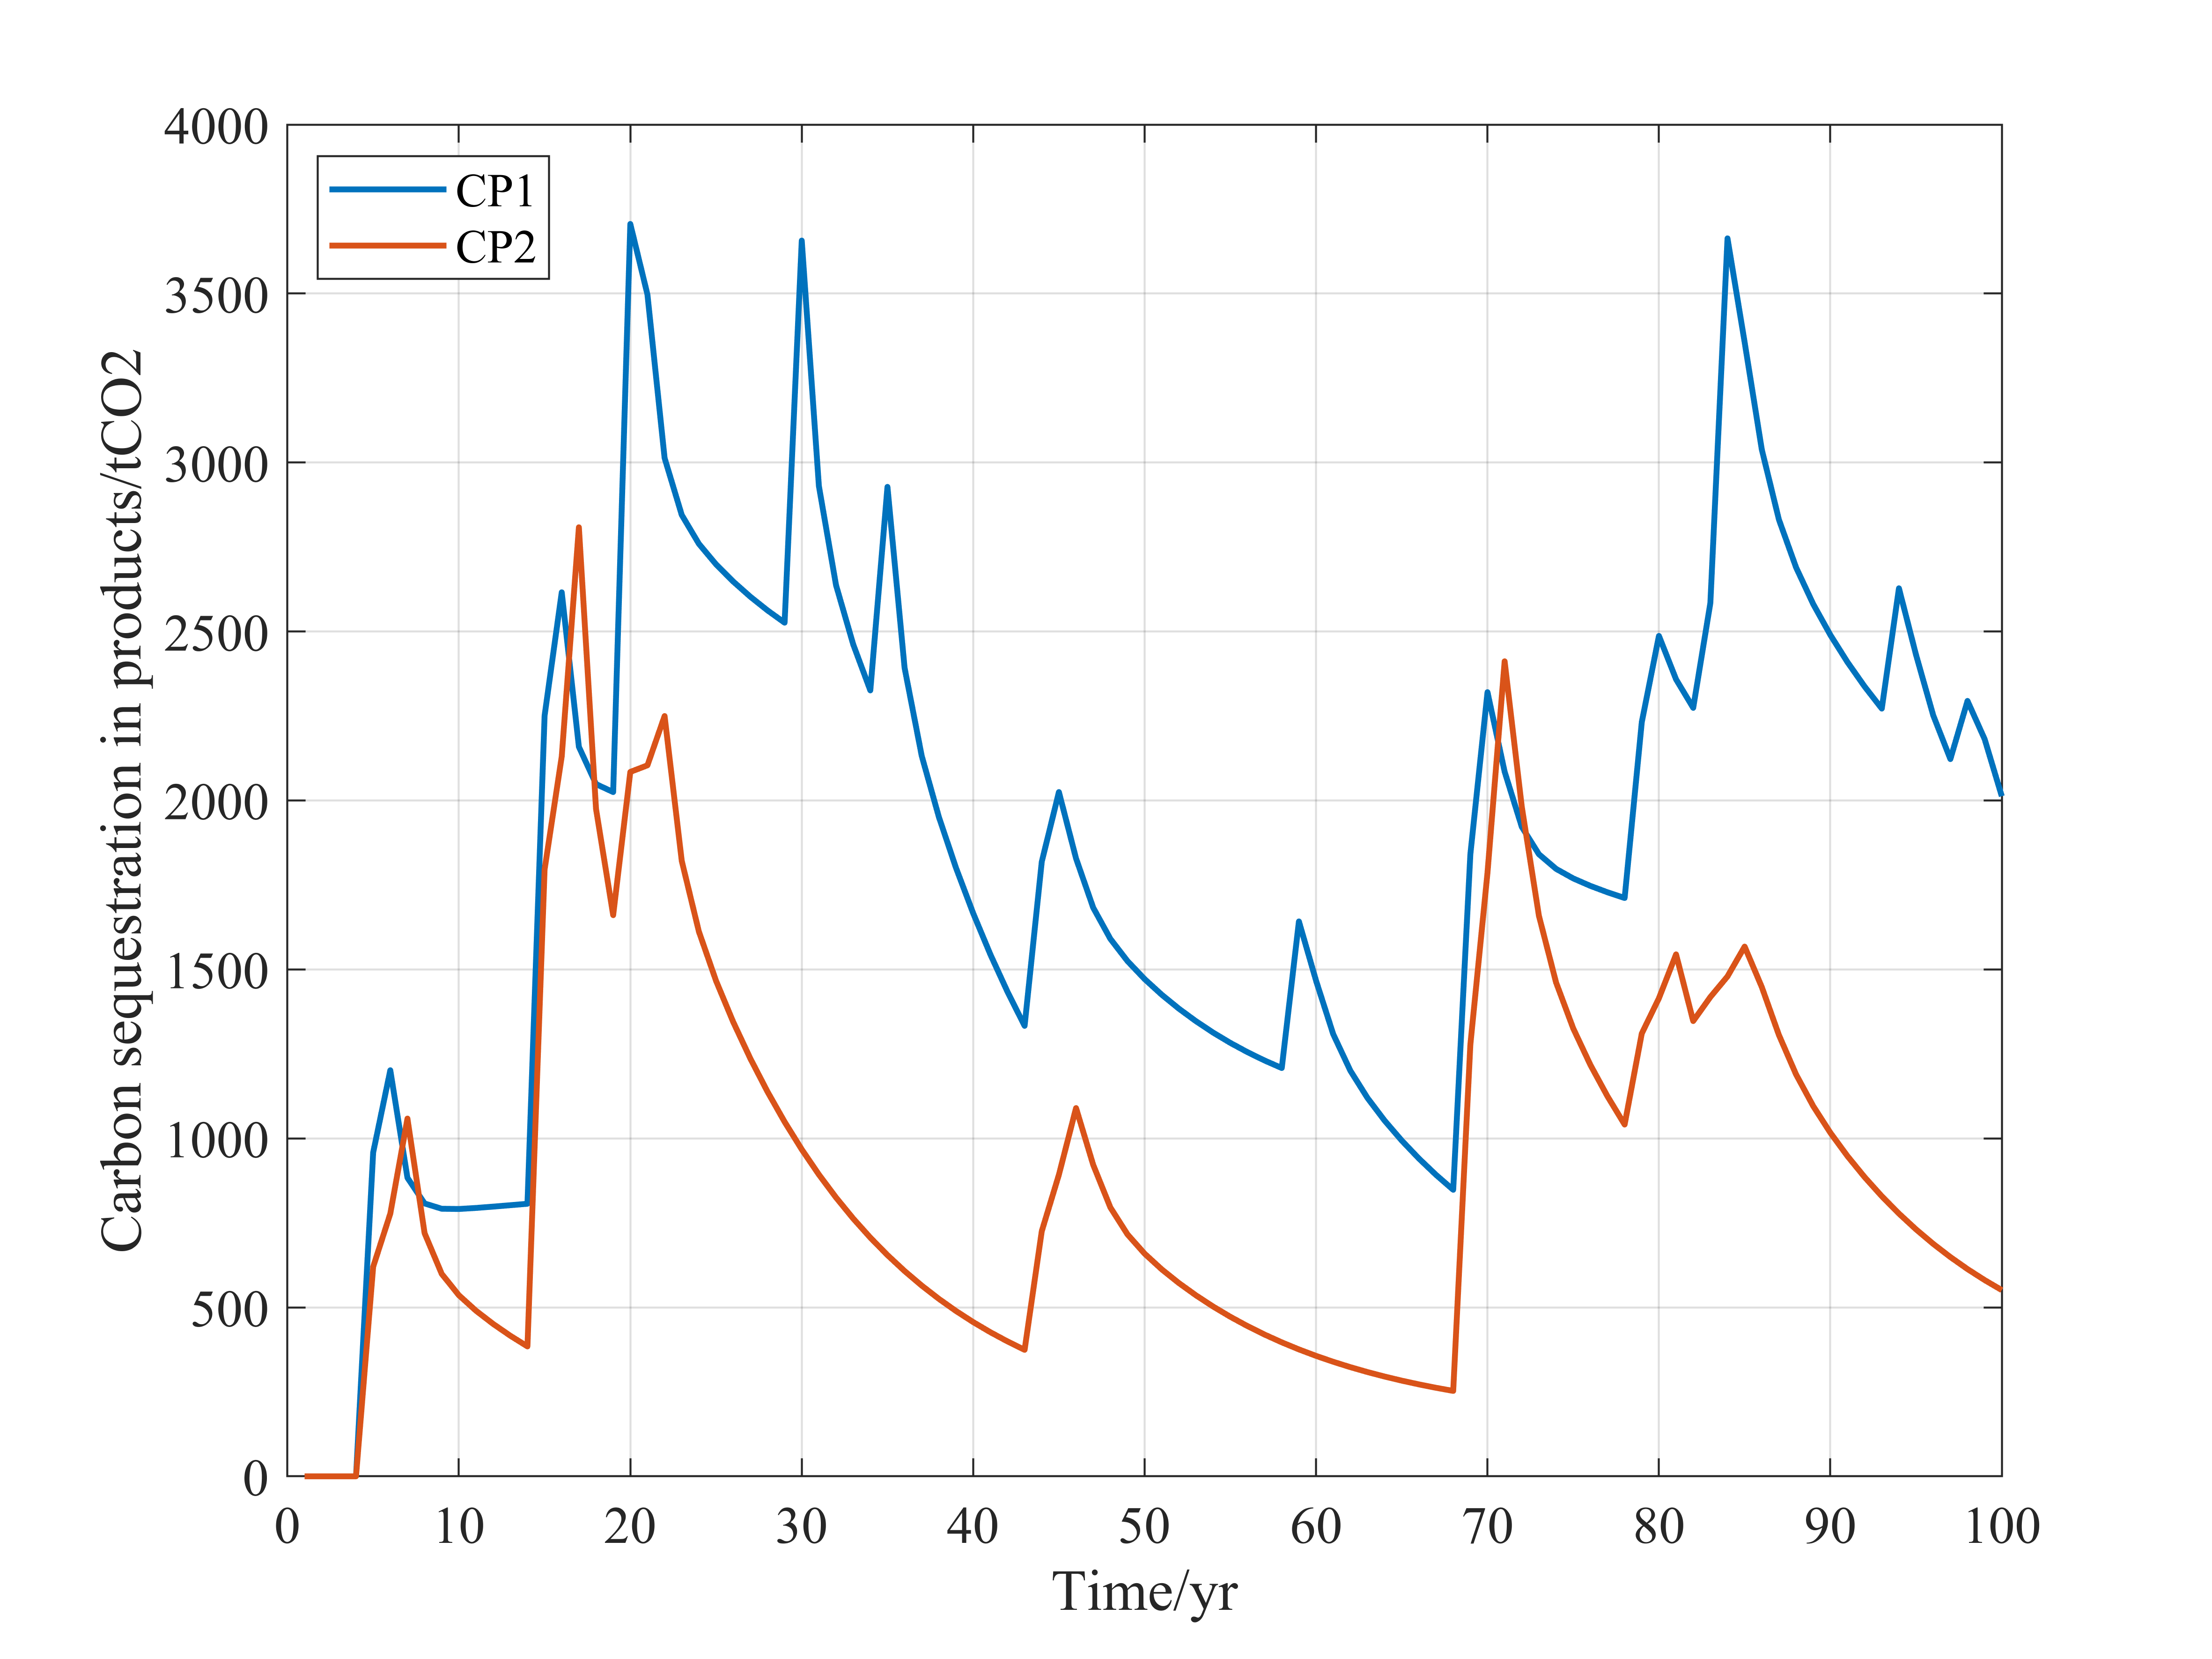
\includegraphics[width=6cm]{figs/Product_S.png}
\caption{Two extremes of product strategy choice.}
\end{minipage}
\begin{minipage}[t]{0.48\textwidth}
\centering
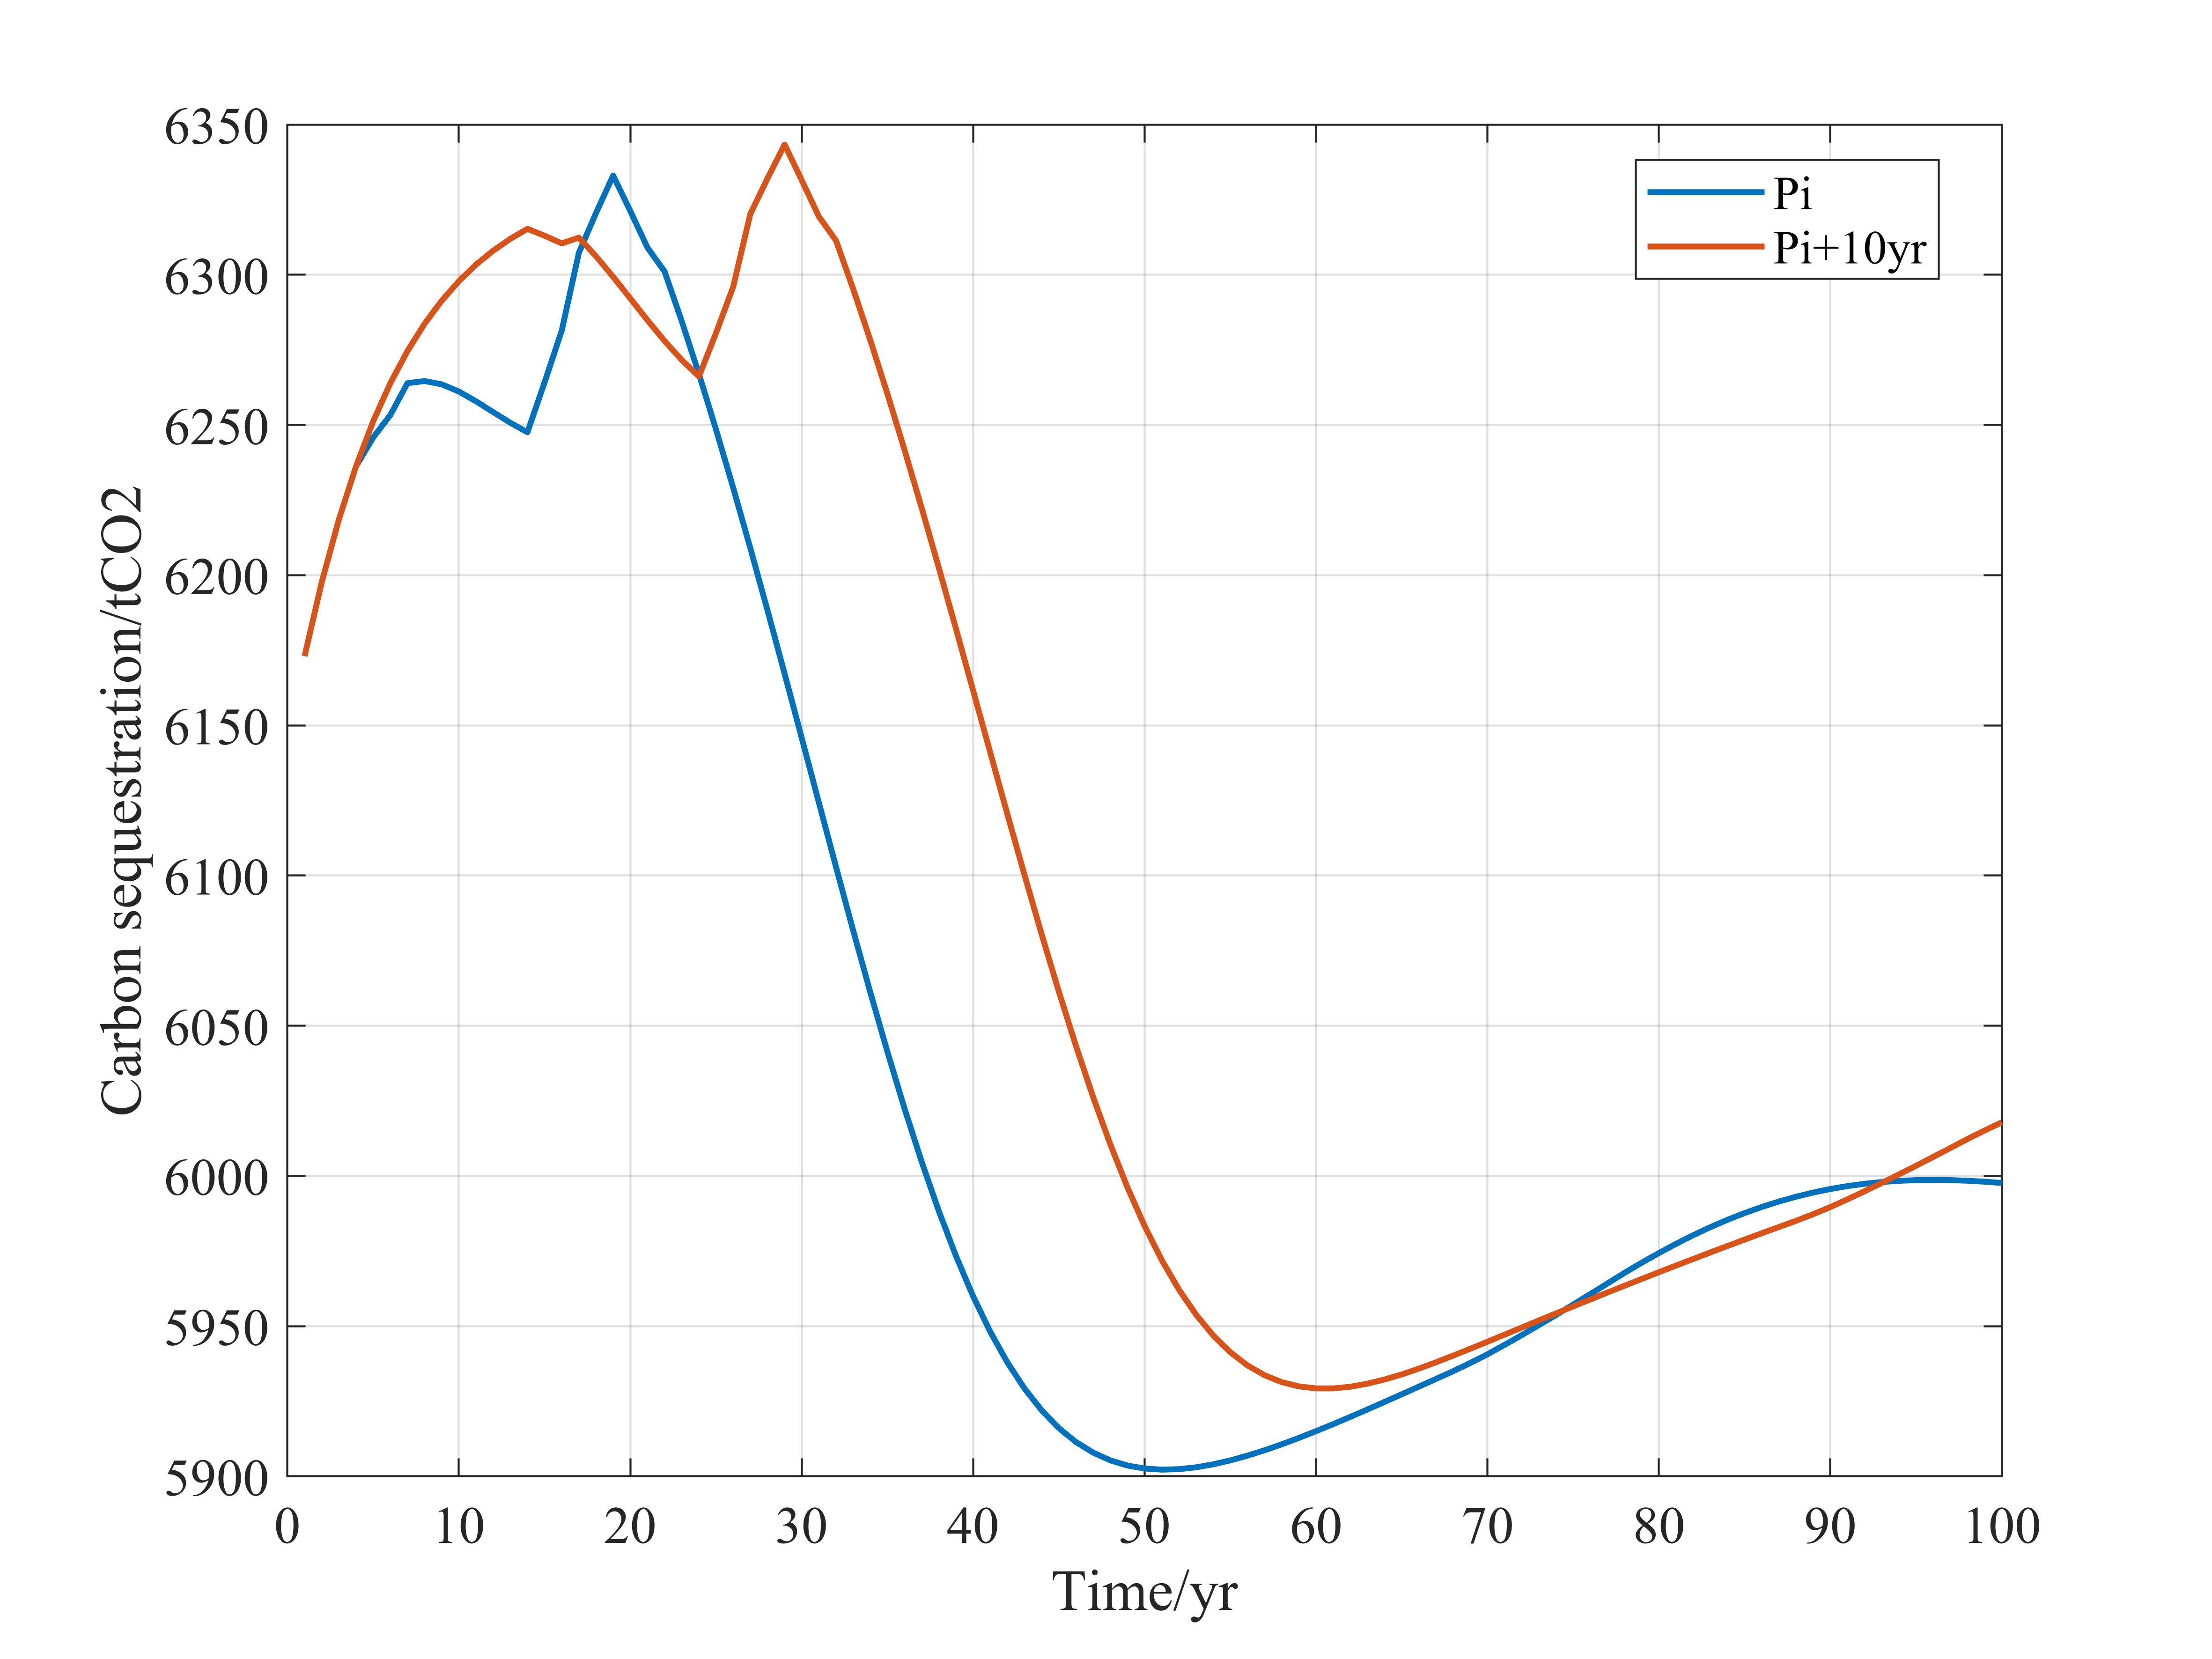
\includegraphics[width=6cm]{figs/Score.png}
\caption{Carbon sequestration of the best management strategy before and after the change of logging period.}
\end{minipage}
\end{figure}

The above analyses lead us to \textbf{the best optimal forest management strategy of pi=0.01 and strategy 2.}

\subsection{Carbon sequestration under optimal forest management strategies}

Based on the existing management strategy for the forest(no logging), we calculated the 100-year carbon sequestration of the current forest at 160.6 tons.

The amount of carbon sequestered by the current optimal strategy and the expected amount of carbon sequestered after the rotation period is extended by 10 years are shown in Figure 8. 

It should be noted that the optimal forest management strategy we derived is only a theoretical reference.

\subsection{Transition strategy after cutting period change.}

In the process of transition from the original scheme to the comprehensive optimal scheme, the change mainly shows that the peak value of carbon sequestration increases. This may be caused by the change in forest product production strategy as trees are closer to maturity and wood properties change.

In order to realize the time line transformation, we give the following transition strategy:

Comparing the two optimal strategy curves, it is found that the two curves are extremely similar. Therefore, we can use smooth transition method. That is, each year for each tree species to increase a certain period of logging, to achieve a steady change in logging cycle.




%! TEX root = ./main.tex

\section{Model Evaluation}

\subsection{Sensitivity Analysis}
The carbon sequestration model's sensitivity to input variables is listed below. Here we use the average carbon sequestration as the output. The model was tested at the best management strategy that we mentioned above. It can be concluded that the model is more sensitive to changes in rotational period $P_i$, but is generally stable  at this point.

\begin{table}[ht]
\centering
\caption{Sensitivity analysis results}
\begin{tabular}{lllll} 
\hline
\multirow{2}{*}{Variables} & \multirow{2}{*}{Fluxes} & \multicolumn{3}{c}{Output}                    \\
                           &                         & Average C(t) & Average CT(t) & Average CP(t)  \\ 
\hline
Felling rate pi            & ±10\%                   & ±0.35\%      & ±0.26\%       & ±0.43\%        \\
Rotation period Pi         & ±1yr                    & ±0.23\%      & ±1.74\%       & ±2.99\%        \\
\hline
\end{tabular}
\end{table}


\subsection{Strength and Weaknesses}
The main advantages of the model are the following.
\begin{itemize}
    \item The tree growth function was fitted by the characteristics of the previous woods growth, reflecting the actual situation under local growth conditions.
    \item Tree mortality and the way the product is disposed of after use are taken into account, so the model reflects the impact of the current social dimension. 
    \item The selected indicators are easy to obtain and the overall design of the model is relatively simple. 
\end{itemize}

However, the model also has shortcomings. 
\begin{itemize}
    \item Many special cases are ignored for the sake of simplicity and easy availability of data and models.
    \item There are still some problems in the setting of social indicators, which lead to the abandonment of indicators due to their insignificance in the actual calculation process. 
    \item The model is only suitable for quantitative analysis of small scale forestland. Large-scale analysis requires the application of remote sensing models.
\end{itemize}




%! TEX root = ./main.tex

\section{Newspaper Article: More logging, more fixed carbon? Reasonable!}

If someone claiming to be a researcher told you that it would be better for the environment to cut down a section of forest near your home, would you simply call him "pseudoscience" and suspect that he was just trying to make money?

As we all know, forest resources are one of the most important resources on earth and are the basis of biological diversity. Forests can adjust the climate, water and soil conservation, prevent and reduce drought and flood, sand, hail and other natural disasters, as well as purify the air, eliminate noise and other functions.

At a time of heightened concern about climate change, the importance of forests is self-evident. Forests play an important role in sequestering carbon dioxide. Through photosynthesis, trees can absorb a lot of carbon dioxide and release oxygen, alleviating the greenhouse effect.

But in real life, forests are also important resources for our life and production. The carbon sequestered by forests can be converted into resources such as food and wood. We get wood and food from forests to make the things we need to live and produce. At a time when human society is expanding rapidly, humans may also be cutting down forests to promote tourism or make more space for human activity.

\begin{figure}[htp]
    \centering
    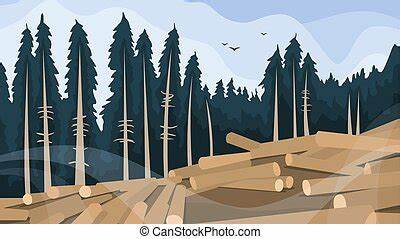
\includegraphics[width=13cm]{figs/logging.jpg}
    \caption{Deforestation.}
    \label{fig:my_label}
\end{figure}

In the traditional view, deforestation is to sacrifice the ecological environment for economic gain. But recent mathematical analysis has led us to a surprising result: proper logging practices can not only improve economic efficiency, but also increase carbon sequestration!
The reason is quite simple: forest products themselves fix part of the carbon, which is basically constant in its service life, and when it reaches its service life, part of the carbon will be returned to the soil by landfill rather than all discharged into the atmosphere. And the land that has been cut down is often replanted with new trees, which also sequester more carbon. Simply put, proper logging strategies can sequester more carbon per unit of land, both in the form of forest products and newly planted trees. That's something you can't do just by using the land for trees.

However, it is important to clarify that we do not support blind overcutting; there is a limit to cutting. We need to find the best balance for trade-offs in time and quantity.

1. Set reasonable rotation period and felling ratio.

2. Set a reasonable proportion of products. Forest products can often be used in a variety of forms to produce a variety of goods, and we can pursue the best strategy by controlling the tree species, location and age of trees harvested.

We recommend that communities further optimize their forest management practices in conjunction with the forest evaluation system, taking into account the ecological, economic, social and sustainability dimensions to achieve a "four best" forest.

Glossary:

Carbon Sequestration: the process of capturing and storing carbon dioxide from the atmosphere.


%! TEX root = ./main.tex

\section{Conclusion}

Forests have a critical impact on global climate change. Therefore, the carbon sequestration capacity of forests should receive focused attention. We developed a carbon sequestration models and a Multi-aspect Decision Model of Forest Management using various methods such as biomass method, entropy weight method, linear fitting method, and cluster analysis method for estimating the carbon sequestration of forests and the comprehensive value of forests. We selected the forest land in Hunan Province as an example analysis, and presumed that its carbon sequestration under the existing management strategy is 160.6 ton. Meanwhile, we proposed to adjust the logging rate to 0.01 and the production strategy to maximize the production of sawn timber, taking into account its natural condition. A smooth transition model was also proposed as a transition strategy based on the change of cutting period. A science-based news article was eventually written to disseminate the study results and provide solutions for community forest management strategies.

%! TEX root = ./main.tex

\newpage

\section{Appendixes}

\subsection{A: Codes}
Below is the source code for carbon sequestration model. Since all three species share the same algorithm, we only represent the source codes for $Choerospondias$.
\begin{lstlisting}
function [CT,CP,C,x] = Task(p,choice,year)
    j = sym('j');
    t = sym('t');
    mu1 = 0.5259; eta1 = 0.1764; rho1 = 0.596;
    average_D1 = 16.86-1.25; N1 = 12600;
    T1 = 35; p1 = p; P1 = 40+year;
    q = 0.334; r = 0.0912;
    Kc = 0.5;
    L1 = 15; Pr1 = 5300;
    if choice == 1
        alpha1 = 0.8*mu1; beta1 = 0; gamma1 = 0.2*mu1+eta1;
    else
        alpha1 = 0; beta1 = 0.8*mu1; gamma1 = 0.2*mu1+eta1;
    end
    
    fit_func = fittype('c/(1+a*exp(-b*t))', 'independent', 't',
    'coefficients', {'a','b','c'});
    raw_D1 = [0 4.650302778 9.912501403 13.17246799 14.9256427
    15.89324511 16.69899162 17.081377]';
    j1 = [0:5:35]';
    cfun_D1 = fit(j1, raw_D1, fit_func);

    raw_H1 = [0 6.21600482 12.83876406 14.10135112 14.79148078
    14.95318602 15.40840566 15.64705269]';
    j1 = [0:5:35]';
    cfun_H1 = fit(j1, raw_H1, fit_func);

   BM1 = @(j) 0.0001*(pi*(cfun_H1.c/(1+cfun_H1.a*exp(-cfun_H1.b*j)))
   *(cfun_D1.c/(1+cfun_D1.a*exp(-cfun_D1.b*j)))^2*rho1)/(4*mu1);

   N1==symsum((cfun_D1.c/(1+cfun_D1.a*exp(-cfun_D1.b*j)))*N1*m1
   *(1-m1)^(j-1),j,1,T1-1)+(cfun_D1.c/(1+cfun_D1.a*exp(-cfun_D1.b*T1)))*N1*(1-m1)^(T1-1);
   m1 = vpasolve(eqn1,m1,0.00558);
   m1 = m1(imag(m1)==0 & real(m1)<1);

    n1 = zeros(200,200);
    CT1 = zeros(1,200);
    for j = 1:T1
        if j == T1
            n1(j,0+1) = N1*(1-m1)^(j-1);
        else
            n1(j,0+1) = N1*m1*(1-m1)^(j-1);
        end
    end
    for t = 1:100
        for j = 1:T1+t
            if j == 1
                n1(j,t+1) = N1*m1+sum(n1(P1-1:T1+t,t))*(1-m1)*p1;
            elseif j >= P1
                n1(j,t+1) = n1(j-1,t)*(1-m1)*(1-p1);
            else
                n1(j,t+1) = n1(j-1,t)*(1-m1);
            end
        end
        for j = 1:T1+t
            CT1(1,t) = CT1(1,t) + Kc*BM1(j)*n1(j,t+1);
        end
    end
    ... ...
    CT = CT1 + CT3 + CT3;
    
    CP1 = zeros(1,200);
    H1 = zeros(1,200);
    for t = 1:100
        for j = P1:t+T1
            H1(1,t+L1) = H1(1,t+L1)+n1(j-1,t)*(1-m1)*p1*BM1(j);
        end
        CP1(1,t) = Kc*(sum(alpha1*H1(1,t+L1-L1:t+L1))
        +sum(beta1*H1(1,t+L1-L2:t+L1))+sum(gamma1*H1(1,t+L1-L3:t+L1)));
        for j = 1:t+L1-L1
            CP1(1,t) = CP1(1,t) + Kc*alpha1*q*H1(1,j)*(exp(-r*(t-j-L1)));
        end
        for j = 1:t+L1-L2
            CP1(1,t) = CP1(1,t) + Kc*beta1*q*H1(1,j)
            *(exp(-r*(t-j-L2)));
        end
    end
    ... ...
    CP = CP1 + CP2 + CP3;
    
    C = CT + CP;
end


\end{lstlisting}


\subsection{B: Data}

\begin{table}[ht]
\centering
\caption{DBH and height variations of different tree species}
\begin{tabular}{lllllll} 
\hline
\multirow{2}{*}{Age [yr]} & \multicolumn{3}{c}{Diameter at breast-height [cm]} & \multicolumn{3}{c}{Height [m]}      \\
                          & Choerospondias & Taiwania & Toona                  & Choerospondias & Taiwania & Toona   \\ 
\hline
0                         & 0              & 0        & 0                      & 0              & 0        & 0       \\
5                         & 4.650          & 1.570    & 2.488                  & 6.216          & 2.507    & 4.798   \\
10                        & 9.913          & 9.211    & 5.155                  & 12.839         & 8.047    & 7.281   \\
15                        & 13.172         & 14.326   & 8.356                  & 14.101         & 13.630   & 10.664  \\
20                        & 14.926         & 15.505   & 12.194                 & 14.791         & 15.017   & 15.374  \\
25                        & 15.893         & 18.244   & 14.747                 & 14.953         & 17.427   & 19.125  \\
30                        & 16.699         & 20.540   & 15.900                 & 15.408         & 18.453   & 21.863  \\
35                        & 17.081         & 22.082   & 16.890                 & 15.647         & 20.347   & 23.282  \\
40                        & -              & 23.317   & 17.453                 & -              & 21.423   & 23.707  \\
\hline
\end{tabular}
\end{table}

\begin{table}[ht]
\centering
\begin{tabular}{llll} 
\hline
\multirow{2}{*}{Component} & \multicolumn{3}{l}{Biomass proportion [\%]}  \\
                           & Choerospondias & Taiwania & Toona            \\ 
\hline
Branches                   & 17.64          & 16.32    & 18.01            \\
Leaves                     & 7.66           & 6.49     & 7.51             \\
Root system                & 22.11          & 22.54    & 23.62            \\
Trunk with bark            & 52.59          & 54.65    & 50.86            \\
\hline
\end{tabular}
\end{table}

\begin{table}[ht]
\centering
\caption{Statistics of tree species at site}
\begin{tabular}{lllll}
\hline
               & \makecell{Number\\ density [hm2]} & \makecell{Average\\ BDH [cm]} & \makecell{Average\\ height [m]} & \makecell{Trunk\\ density [g/cm3]}  \\
\hline
Choerospondias & 1260                   & 16.86            & 15.65              & 0.596                    \\
Taiwania       & 1140                   & 23.01            & 21.27              & 0.358                    \\
Toona          & 870                    & 17.21            & 23.57              & 0.475                    \\
\hline
\end{tabular}
\end{table}

\newpage
%\bibliographystyle{ieeetr}
\clearpage
\phantomsection
\addcontentsline{toc}{section}{References} %向目录中添加条目,以章的名义

\printbibliography

%%%%%%%%%%%%%%%%%%%%%%%%%%%%%%
\end{document}
\end